\section{Problem Analysis}
% motivation for creating this theme
\begin{frame}{Main Challenges}{Object Variations}
\begin{columns}
    \column{0.2\textwidth}
        \begin{block}{Intra-class}
        \begin{itemize}
            \item Texture
            \item Colour
            \item Shape
            \item Size
        \end{itemize}
            

        \end{block}
    \column{0.4\textwidth}
        \begin{figure}
            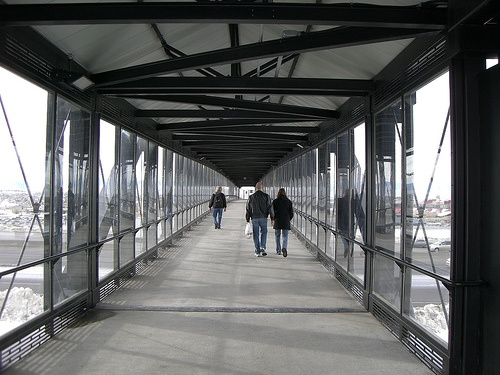
\includegraphics[width=0.7 \textwidth]{figs/000066.jpg}
        \end{figure}
        \begin{figure}
            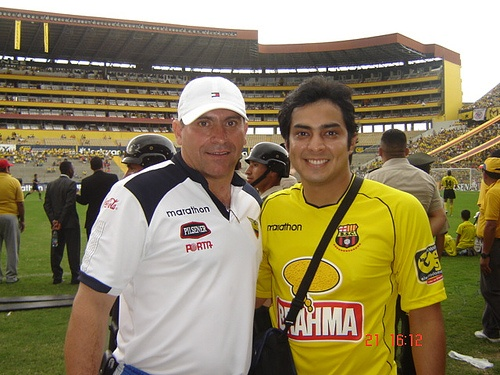
\includegraphics[width=0.7 \textwidth]{figs/000076.jpg}
        \end{figure}

    \column{0.4\textwidth}
        \begin{figure}
            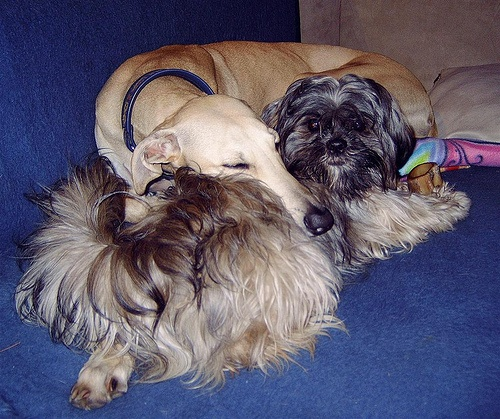
\includegraphics[width=0.7 \textwidth]{figs/000078.jpg}
        \end{figure}

    \end{columns}
\end{frame}

\begin{frame}{Main Challenges}{Object Variations}
\begin{columns}
    \column{0.2\textwidth}
        \begin{block}{Inter-class}
        \begin{itemize}
            \item Texture
            \item Colour
            \item Shape
            \item Size
        \end{itemize}
            

        \end{block}
    \column{0.4\textwidth}
        \begin{figure}
            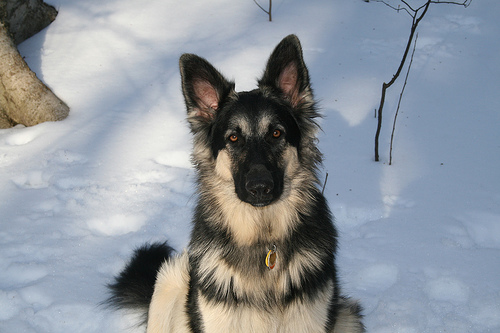
\includegraphics[width=1.0 \textwidth]{figs/germanshepherd.jpeg}
        \end{figure}
    \column{0.4\textwidth}
        \begin{figure}
            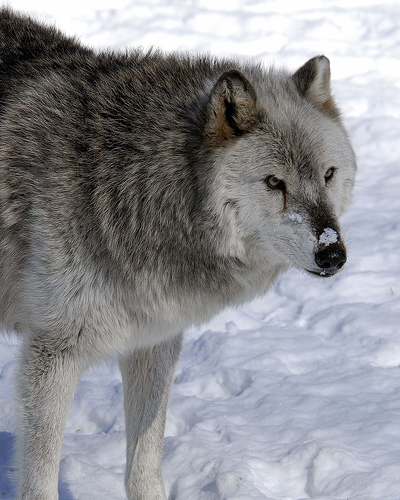
\includegraphics[width=0.7 \textwidth]{figs/wolf.jpeg}
        \end{figure}
    \end{columns}
\end{frame}

\begin{frame}{Main Challenges}{Image Variations}
\begin{columns}
    \column{0.3\textwidth}
        \begin{block}{Intra-class}
        \begin{itemize}
            \item Lighting
            \item Viewpoint
            \item Occlusion
            \item Clutter
            \item Quality
        \end{itemize}
            

        \end{block}
    \column{0.35\textwidth}
        \begin{figure}
            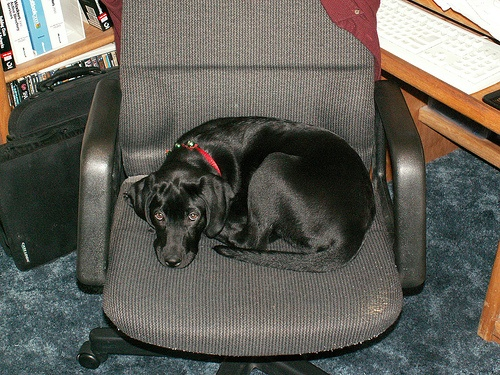
\includegraphics[width=0.7 \textwidth]{figs/000063.jpg}
        \end{figure}
        \begin{figure}
            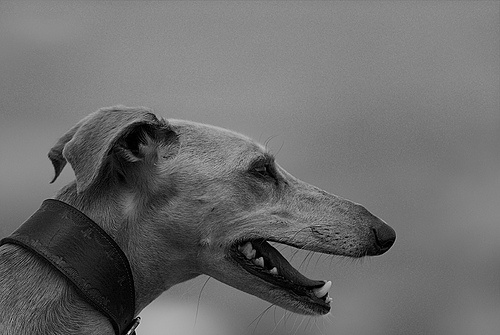
\includegraphics[width=0.7 \textwidth]{figs/000065.jpg}
        \end{figure}

    \column{0.35\textwidth}
        \begin{figure}
            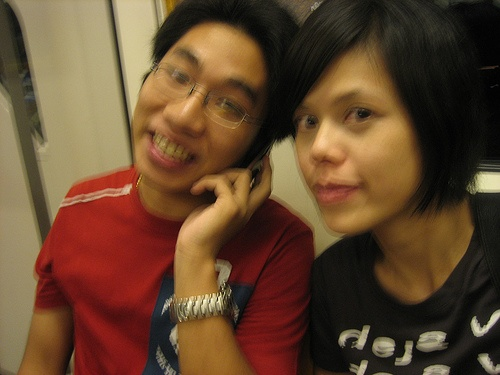
\includegraphics[width=0.7 \textwidth]{figs/000323.jpg}
        \end{figure}
        \begin{figure}
            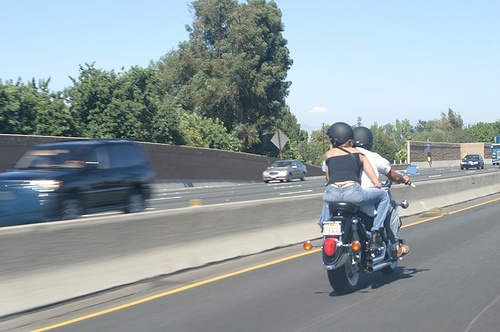
\includegraphics[width=0.7 \textwidth]{figs/000579.jpg}
        \end{figure}

    \end{columns}
\end{frame}

\begin{frame}{Main Challenges}{}
        \begin{block}{Computational-complexity and scalability-related}
        \begin{itemize}
            \item Potential scale of object detection
            \item Robustness-related complexity
            \item Change in problem over time
        \end{itemize}
            

        \end{block}
\end{frame}

\begin{frame}{State-of-the-art}{}
        \begin{block}{Tackling the key challenges}
        \begin{itemize}
            \item Region-Based
            \begin{itemize}
                \item R-CNN, Fast R-CNN, Faster R-CNN
            \end{itemize}
            \item Fully-Convolutional Networks
            \begin{itemize}
                \item R-FCN
            \end{itemize}
            \item Ensemble Methods
            \begin{itemize}
                \item All leading methods on benchmarks
                \item Trained on different subsets of data, architectures, loss functions, etc
            \end{itemize}
        \end{itemize}            
        \end{block}
\end{frame}

\begin{frame}{Problem Statement}{}
        \begin{block}{Goal}
            \begin{itemize}
                \item Localise \& classify relevant objects in an image
            \end{itemize}            
        \end{block}
        \begin{block}{Challenges}
            \begin{itemize}
                \item Robustness-related
                \item Computational complexity \& scalability-related
            \end{itemize}            
        \end{block}
        \begin{block}{State-of-the-art}
            \begin{itemize}
                \item All leading methods in benchmarks use ensemble methods
                \item Trained on different variations of data, architectures, loss functions, etc
            \end{itemize}            
        \end{block}

        \textit{How can specific robust-related challenges be addressed in a CNN-based object detector with the aid of ensemble methods?}
\end{frame}
